\chapter{Introdu\c{c}\~{a}o te\'{o}rica}
Os transformadores (chamados tamb\'{e}m de trafos) s\~{a}o utilizados numa gama muito variada de aplica\c{c}\~{o}es de processamento de informa\c{c}\~{a}o e de energia el\'{e}ctrica. Salientam-se, entre outras, a eleva\c{c}\~{a}o e a redu\c{c}\~{a}o da tens\~{a}o e do n\'{u}mero de fases em redes de transporte e distribui\c{c}\~{a}o de energia el\'{e}ctrica, a redu\c{c}\~{a}o da tens\~{a}o ou da corrente em instrumentos de medida, a adapta\c{c}\~{a}o de imped\^{a}ncias em amplificadores sintonizados em aplica\c{c}\~{o}es de radiofrequ\^{e}ncia e frequ\^{e}ncia interm\'{e}dia, a adapta\c{c}\~{a}o de resist\^{e}ncias em aplica\c{c}\~{o}es \'{a}udio, ou simplesmente o isolamento galv\^{a}nico entre partes de um mesmo circuito el\'{e}ctrico.
O princ\'{\i}pio b\'{a}sico de funcionamento de um transformador \'{e} o fen\^{o}meno conhecido como indu\c{c}\~{a}o eletromagn\'{e}tica: quando um circuito \'{e} submetido a um campo magn\'{e}tico vari\'{a}vel, aparece nele uma corrente el\'{e}trica cuja intensidade \'{e} proporcional \`{a}s varia\c{c}\~{o}es do fluxo magn\'{e}tico.

\section{Simbologia}
Tradicionalmente, quando representados em diagramas el\'{e}tricos, os transformadores possuem simbologias que expressam seus dois enrolamentos (prim\'{a}rio e secund\'{a}rio) como pode-se observar na ilustra\c{c}\~{a}o a seguir:

Outras simbologias s\~{a}o apresentadas em diversas literaturas dispon\'{\i}veis, no entanto, as simbologias acima apresentadas s\~{a}o as mais usuais para transformadores monof\'{a}sicos. //

\centerline{\begin{minipage}[c]{\textwidth}
\centering
\noindent
        \captionof{figure}{Representa\c{c}\~{a}o do circuito com o diodo (ideal) polarizado inversamente}
		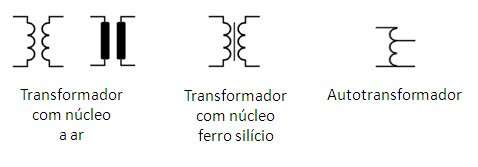
\includegraphics[width=0.5\textwidth]{Imagens/Desenvolvimento-Imagem1.jpg}
		\legend{Fonte:lelele}
		\label{fig:image11}
 \end{minipage}}

\centerline{\begin{minipage}[c]{\textwidth}
\centering
\noindent
        \captionof{figure}{Representa\c{c}\~{a}o do circuito com o diodo (ideal) polarizado inversamente}
		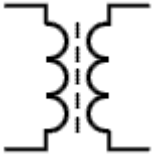
\includegraphics[width=0.5\textwidth]{Imagens/Desenvolvimento-Imagem2.png}
		\legend{Fonte:lelele}
		\label{fig:image11}
 \end{minipage}}

\section{Caracter\'{\i}sticas construtivas de um Trafo}

Um transformador simples pode ser dividido em tr\^{e}s principais partes:
\begin{itemize}
  \item Enrolamento Prim\'{a}rio;
  \item Enrolamento Secund\'{a}rio;
  \item N\'{u}cleo.
\end{itemize} //

\centerline{\begin{minipage}[c]{\textwidth}
\centering
\noindent
        \captionof{figure}{Representa\c{c}\~{a}o do circuito com o diodo (ideal) polarizado inversamente}
		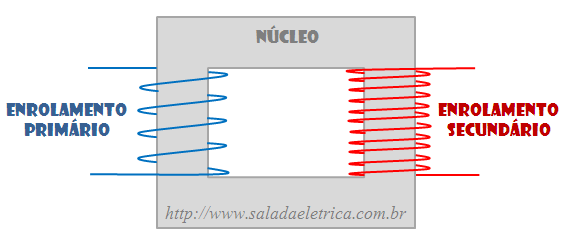
\includegraphics[width=0.5\textwidth]{Imagens/Desenvolvimento-Imagem3.png}
		\legend{Fonte:lelele}
		\label{fig:image11}
 \end{minipage}}

Os transformadores, na sua forma mais simples (figura 3), consistem de dois enrolamentos de fio (o prim\'{a}rio e o secund\'{a}rio), que geralmente envolvem os bra\c{c}os de um quadro met\'{a}lico (o n\'{u}cleo). Quando uma corrente alternada \'{e} aplicada ao prim\'{a}rio produz um campo magn\'{e}tico proporcional \`{a} intensidade dessa corrente e ao n\'{u}mero de espiras do enrolamento (n\'{u}mero de voltas do fio em torno do bra\c{c}o met\'{a}lico). Atrav\'{e}s do metal, o fluxo magn\'{e}tico quase n\~{a}o encontra resist\^{e}ncia e, assim, concentra-se no n\'{u}cleo, em grande parte, e chega ao enrolamento secund\'{a}rio com um m\'{\i}nimo de perdas. Ocorre, ent\~{a}o, a indu\c{c}\~{a}o eletromagn\'{e}tica: no secund\'{a}rio surge uma corrente el\'{e}trica, que varia de acordo com a corrente do prim\'{a}rio e com a raz\~{a}o entre os n\'{u}meros de espiras dos dois enrolamentos. //

\centerline{\begin{minipage}[c]{\textwidth}
\centering
\noindent
        \captionof{figure}{Representa\c{c}\~{a}o do circuito com o diodo (ideal) polarizado inversamente}
		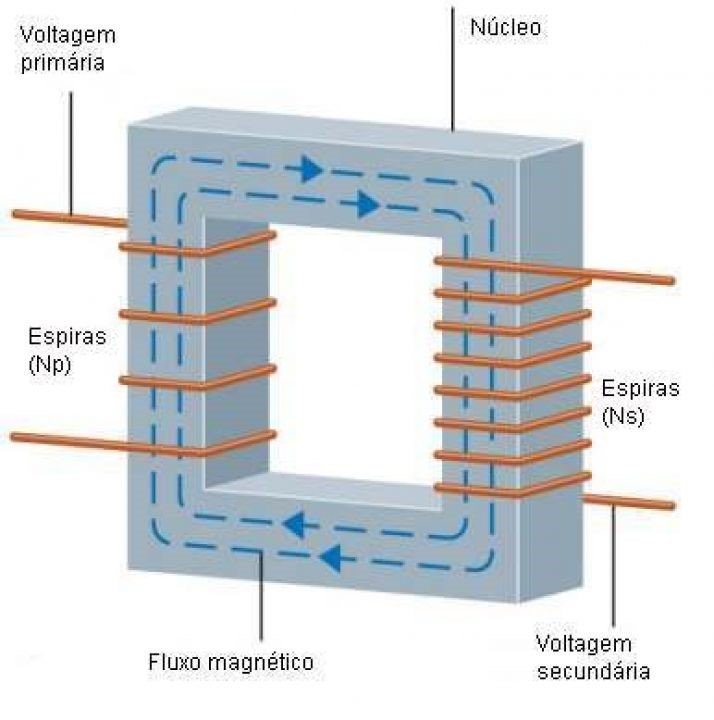
\includegraphics[width=0.5\textwidth]{Imagens/Desenvolvimento-Imagem4.jpg}
		\legend{Fonte:lelele}
		\label{fig:image11}
 \end{minipage}}

A rela\c{c}\~{a}o entre as voltagens no prim\'{a}rio e no secund\'{a}rio, bem como entre as correntes nesses enrolamentos, pode ser facilmente obtida: se o prim\'{a}rio tem Np espiras e o secund\'{a}rio Ns, a voltagem no prim\'{a}rio (Vp) est\'{a} relacionada \`{a} voltagem no secund\'{a}rio (Vs) por Vp/Vs=Np/Ns , e as correntes por Np/Ns=Is/Ip. Por esta proporcionalidade conclu\'{\i}mos que um transformador reduz a tens\~{a}o se o n\'{u}mero de espiras do secund\'{a}rio for menor que o n\'{u}mero de espiras do prim\'{a}rio e vice-verso.

Al\'{e}m das simbologias apresentadas, temos os tipos mais comuns de transformadores com configura\c{c}\~{o}es de bobinas: //

*************** tabel\~{a}o **************** //

\section{Perdas no transformador}

As principais perdas em um transformador ocorrem nos enrolamentos e no n\'{u}cleo. Nos enrolamentos, devido \`{a} resist\^{e}ncia \^{o}hmica do fio, parte da energia e convertida em calor por Efeito Joule, causando perdas denominadas perdas no cobre. No n\'{u}cleo, temos perdas causadas pela revers\~{a}o magn\'{e}tica cada vez que a corrente muda de sentido (Ciclo de Histerese), pela dispers\~{a}o de linhas de campo magn\'{e}tico e pelas correntes parasitas de Foucault, que induzidas no n\'{u}cleo o aquecem, reduzindo o campo principal. Para evitar as correntes de Foucault, o n\'{u}cleo \'{e} constitu\'{\i}do por chapas laminadas, isoladas por um verniz e solidamente agrupadas. Para diminuir as perdas por Histerese o material das chapas \'{e} composto de a\c{c}o-sil\'{\i}cio. Para reduzir a dispers\~{a}o de fluxo, todo o conjunto tem um formato apropriado, onde os enrolamentos prim\'{a}rio e secund\'{a}rio s\~{a}o, atrav\'{e}s de um carretel, colocados na parte central, concentrando dessa maneira as linhas de campo magn\'{e}tico. A Figura 4 mostra um transformador com as caracter\'{\i}sticas construtivas citadas. //


\centerline{\begin{minipage}[c]{\textwidth}
\centering
\noindent
        \captionof{figure}{Representa\c{c}\~{a}o do circuito com o diodo (ideal) polarizado inversamente}
		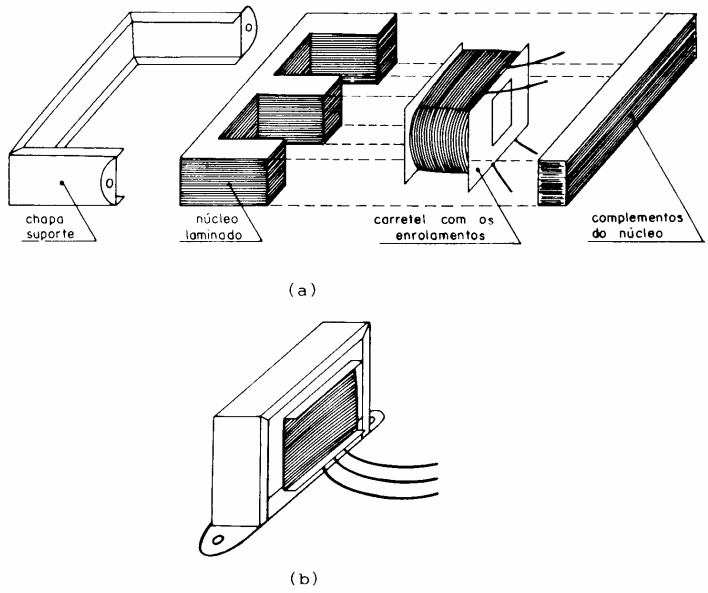
\includegraphics[width=0.5\textwidth]{Imagens/Desenvolvimento-Imagem5.png}
		\legend{Fonte:lelele}
		\label{fig:image11}
 \end{minipage}}

\section{Retificador}

O circuito que transforma a CA em CC, se chama de retificador, ou seja, faz com que a corrente na carga circule em um \'{u}nico sentido. Existem dois tipos de retificadores: Retificador de meia onda e retificador de onda completa.

\subsection{Retificador de Meia Onda}

O diodo tem a caracter\'{\i}stica de conduzir corrente somente num sentido e devido a esta caracter\'{\i}stica unidirecional, o mesmo \'{e} utilizado para retificar. O diodo ideal com polariza\c{c}\~{a}o direta comporta como uma chave fechada e com polariza\c{c}\~{a}o reversa comporta como uma chave aberta. O diodo tem resist\^{e}ncia direta muito baixa e resist\^{e}ncia reversa muito alta. \\

\centerline{\begin{minipage}[c]{\textwidth}
\centering
\noindent
        \captionof{figure}{Representa\c{c}\~{a}o do circuito com o diodo (ideal) polarizado inversamente}
		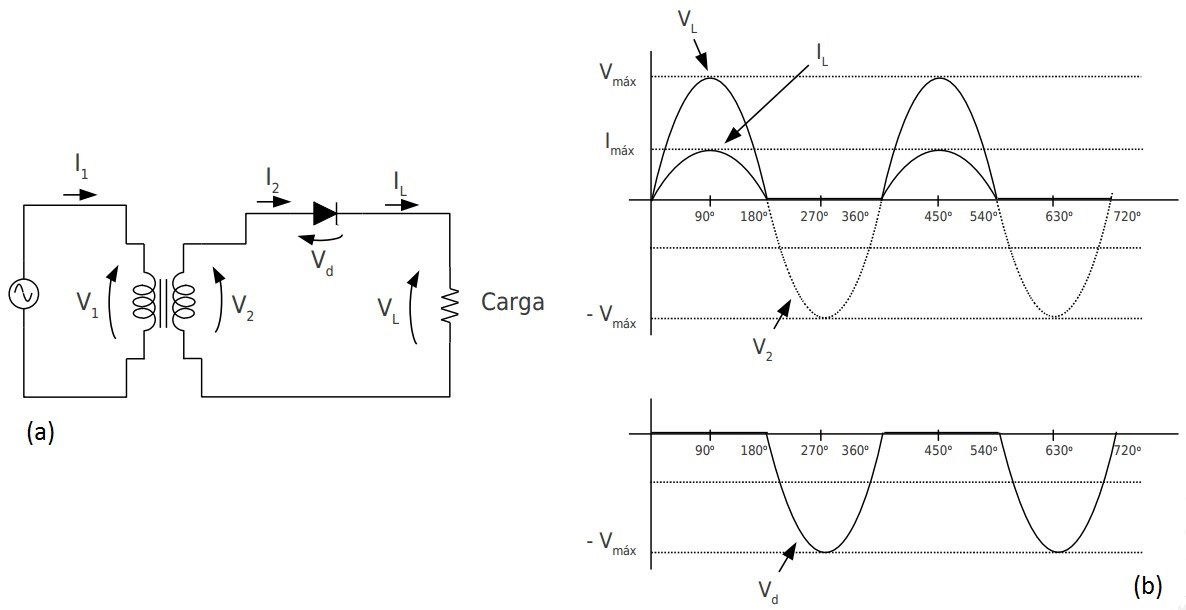
\includegraphics[width=0.5\textwidth]{Imagens/Desenvolvimento-Imagem6.jpg}
		\legend{Fonte:lelele}
		\label{fig:image11}
 \end{minipage}}

\subsubsection{Funcionamento do circuito}
Como a corrente est\'{a} no sentido do diodo, ele estar\'{a} polarizado diretamente e conduz. Tendo assim que a corrente circula passando pelo diodo e carga. Na parte negativa, a corrente inverte o sentido, fazendo com que o diodo esteja polarizado inversamente e n\~{a}o conduz. Tem-se corrente na carga somente nos semiciclos positivos de entrada. Os semiciclos positivos passam para a sa\'{\i}da e os semiciclos negativos ficam no diodo. A freq\"{u}\^{e}ncia de ondula\c{c}\~{a}o na sa\'{\i}da \'{e} igual \`{a} freq\"{u}\^{e}ncia de entrada. O retificador de meia onda tem baixa efici\^{e}ncia.

Para este circuito podemos escrever algumas express\~{o}es importantes para a determina\c{c}\~{a}o das caracter\'{\i}sticas do nosso diodo. Muitas delas n\~{a}o ser\~{a}o demonstradas e simplesmente apresentadas, pois suas demonstra\c{c}\~{o}es necessitam de t\'{e}cnicas matem\'{a}ticas mais avan\c{c}adas. As express\~{o}es s\~{a}o: \\

********** c\'{o}digos gabriel ************ \\

\subsection{Retificador de onda completa em ponte}
O circuito em ponte utiliza quatro diodos ligados conforme mostra a figura 6a. Este circuito utiliza uma transformador de secund\'{a}rio simples, tendo como vantagem a n\~{a}o utiliza\c{c}\~{a}o de um transformador com tape central ou center tape. Na figura 6b temos a seq\"{u}\^{e}ncia de condu\c{c}\~{a}o dos diodos, e na figura 6c as principais formas de onda no circuito. Observe que neste circuito o diodo n\~{a}o possui mais como tens\~{a}o reversa 2V m\'{a}x, e sim a metade deste valor, que em alguns casos \'{e} essencial esta situa\c{c}\~{a}o, pois quanto maior a tens\~{a}o reversa do diodo mais oneroso pode se tornar o circuito. \\

\centerline{\begin{minipage}[c]{\textwidth}
\centering
\noindent
        \captionof{figure}{Representa\c{c}\~{a}o do circuito com o diodo (ideal) polarizado inversamente}
		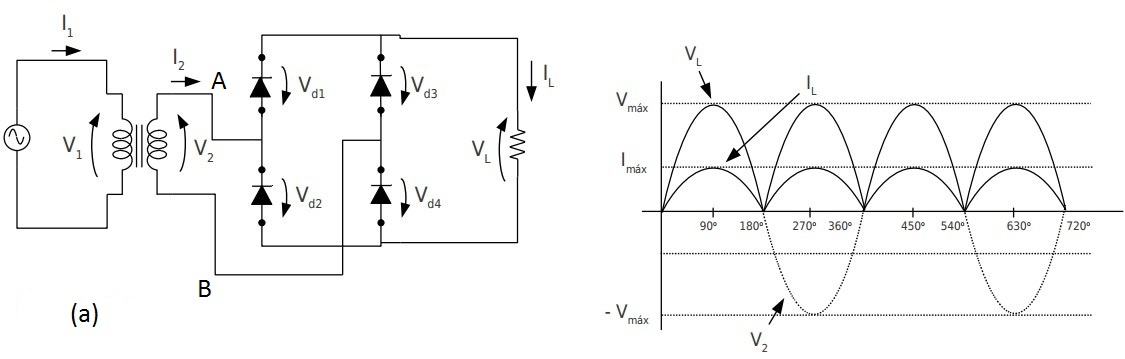
\includegraphics[width=0.5\textwidth]{Imagens/Desenvolvimento-Imagem8.png}
		\legend{Fonte:lelele}
		\label{fig:image11}
 \end{minipage}}

\centerline{\begin{minipage}[c]{\textwidth}
\centering
\noindent
        \captionof{figure}{Representa\c{c}\~{a}o do circuito com o diodo (ideal) polarizado inversamente}
		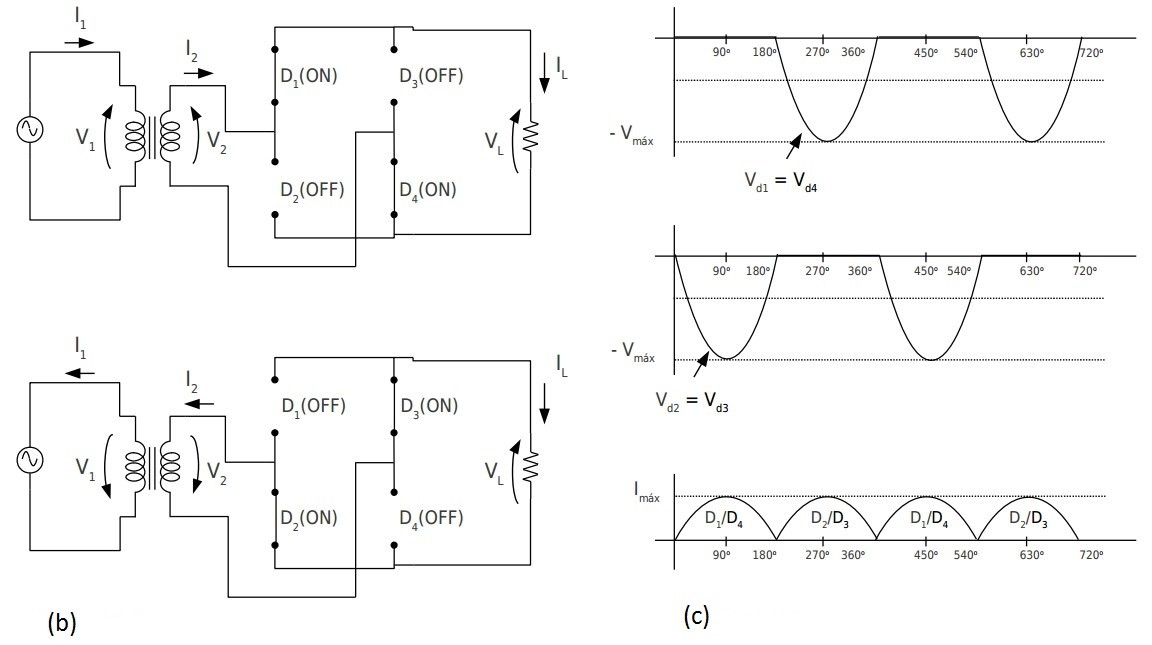
\includegraphics[width=0.5\textwidth]{Imagens/Desenvolvimento-Imagem9.jpg}
		\legend{Fonte:lelele}
		\label{fig:image11}
 \end{minipage}}

\subsubsection{Funcionamento do circuito}
O retificador em ponte dispensa o uso do transformador com tomada central. Com isto, pode-se ter um retificador de onda completa ligado diretamente \`{a} rede el\'{e}trica. Quando A \'{e} positivo em rela\c{c}\~{a}o a B, a corrente sai de A passa por D1, RL, D3 e chega ao ponto B. Quando A \'{e} negativo em rela\c{c}\~{a}o a B, a corrente sai de B passa por D2, RL, D4 e chega ao ponto A. Conduzem somente dois diodos de cada vez. Quando o ponto A \'{e} positivo D1 e D3 conduzem. Quando o ponto A \'{e} negativo D2 e D4 conduzem. Para qualquer polaridade de A ou de B a corrente IL circula num \'{u}nico sentido em RL e por isto, a corrente em RL \'{e} cont\'{\i}nua. Temos somente os semiciclos positivos na sa\'{\i}da. A frequ\^{e}ncia de ondula\c{c}\~{a}o na sa\'{\i}da \'{e} o dobro da frequ\^{e}ncia de entrada.

As express\~{o}es para as tens\~{o}es e correntes nos elementos do circuito e na carga s\~{a}o dadas na tabela a seguir.\\

********** c\'{o}digos gabriel ************ \\

\subsection{Retificador de onda completa com trafo de deriva\c{c}\~{a}o central}
Este circuito, \'{e} apresentado no circuito da figura 7a. Neste circuito temos apenas dois diodos, onde um dos diodos conduz um semiciclo da corrente e o outro diodo conduz o outro semiciclo da corrente. Isto s\'{o} \'{e} poss\'{\i}vel porque o transformador possui uma deriva\c{c}\~{a}o central ou center tape – CT. Na realidade \'{e} como se fosse um transformador com uma prim\'{a}rio e dois secund\'{a}rios ligado sem s\'{e}rie, sendo o ponto de liga\c{c}\~{a}o destes o CT. Desta forma, cada enrolamento ir\'{a} fornecer corrente para um semi ciclo da onda. A figura 7b traz a seq\"{u}\^{e}ncia de condu\c{c}\~{a}o dos diodos como sendo ON para diodo conduzindo e OFF para diodo n\~{a}o conduzindo, e a figura 7c as formas de ondas nos elementos do circuito. \\

\centerline{\begin{minipage}[c]{\textwidth}
\centering
\noindent
        \captionof{figure}{Representa\c{c}\~{a}o do circuito com o diodo (ideal) polarizado inversamente}
		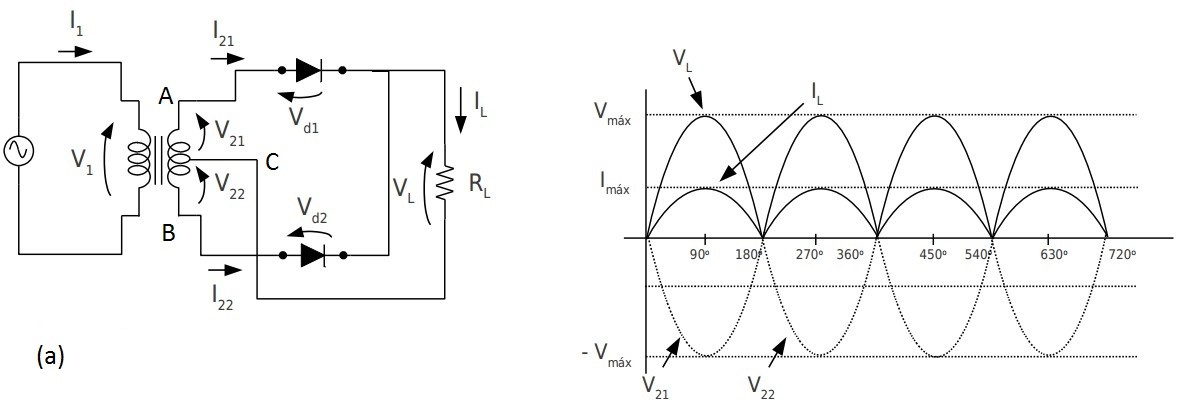
\includegraphics[width=0.5\textwidth]{Imagens/Desenvolvimento-Imagem11.jpg}
		\legend{Fonte:lelele}
		\label{fig:image11}
 \end{minipage}}


\centerline{\begin{minipage}[c]{\textwidth}
\centering
\noindent
        \captionof{figure}{Representa\c{c}\~{a}o do circuito com o diodo (ideal) polarizado inversamente}
		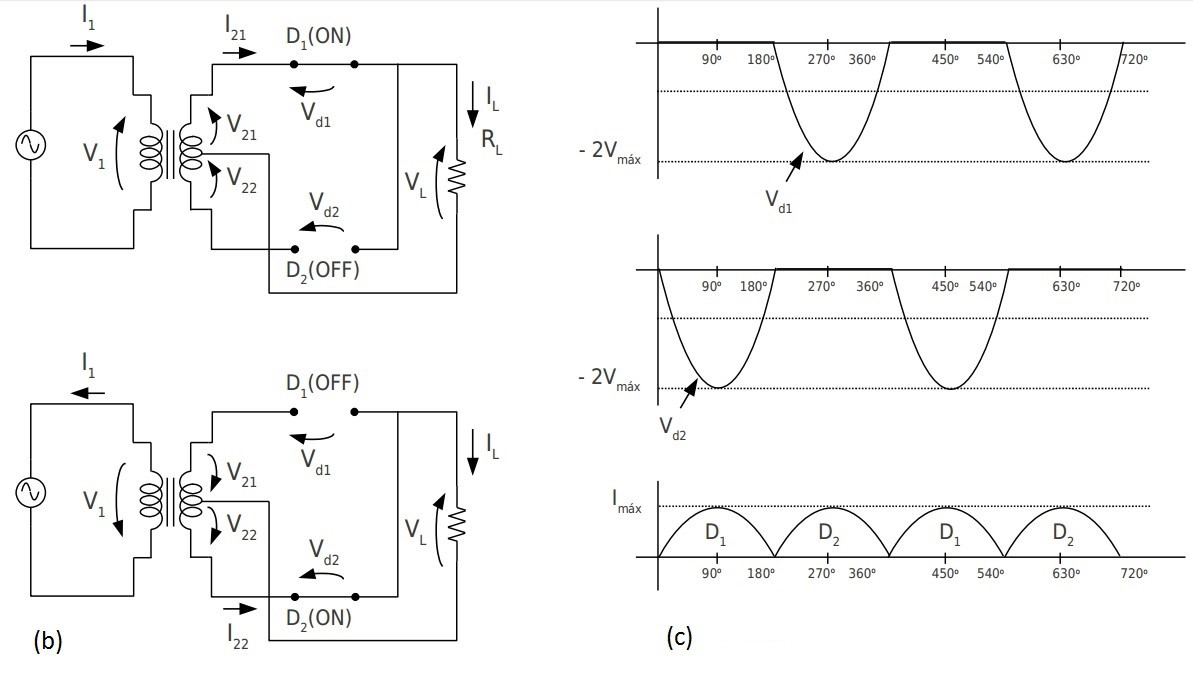
\includegraphics[width=0.5\textwidth]{Imagens/Desenvolvimento-Imagem12.jpg}
		\legend{Fonte:lelele}
		\label{fig:image11}
 \end{minipage}}

 \subsubsection{Funcionamento do circuito}
 Este circuito \'{e} tamb\'{e}m denominado de retificador de onda completa convencional. H\'{a} uma defasagem de 180º entre as tens\~{o}es de sa\'{\i}da do transformador, VA e VB. As tens\~{o}es VA e VB s\~{a}o medidas em rela\c{c}\~{a}o ao ponto C (0V ). Quando A \'{e} positivo, B \'{e} negativo, a corrente sai de A passa por D1 e RL e chega ao ponto C. Quando A \'{e} negativo, B \'{e} positivo, a corrente sai de B passa por D2 e RL e chega ao ponto C. Para qualquer polaridade de A ou de B a corrente IL circula num \'{u}nico sentido em RL e por isto, a corrente em RL \'{e} cont\'{\i}nua. Temos somente os semiciclos positivos na sa\'{\i}da. A frequ\^{e}ncia de ondula\c{c}\~{a}o na sa\'{\i}da \'{e} o dobro da frequ\^{e}ncia de entrada.
Da mesma forma podemos escrever as express\~{o}es para as tens\~{o}es e correntes nos elementos do circuito e na carga:

********** c\'{o}digos gabriel ************ \\ 